
\section{Experimental details and ablations for section~\ref{sec:calibrating_models}}

\label{sec:calibrating_models_appendix_experiments}

We give more experimental details for our CIFAR-10 experiment, show experimental results for top-label calibration in ImageNet and CIFAR-10, and give details and results for our synthetic experiments. Note that the code is available in the supplementary folder for completeness.

\textbf{Experimental details}: We detail our experimental protocol for CIFAR-10 first. The CIFAR-10 validation set has 10,000 data points. We sampled, with replacement, a recalibration set of 1,000 points. In our theoretical approach and analysis, we split up these sets into multiple parts. For example, we used the first part for training a function, second part for bin construction, third part for binning. In practice, using the same set for all three steps worked out better, for both histogram binning and \ourcal{}. We believe that there may be theoretical justification for merging these sets, although we leave that for future work. For the marginal calibration experiment we ran either \ourcal{} (we fit a sigmoid in the function fitting step) or histogram binning. We calibrated each of the $K$ classes seprately as described in Section~\ref{sec:formulation}, and measured the marginal calibration error on the entire set of 10K points. We repeated this entire procedure 100 times, and computed mean and 90\% confidence intervals.

\begin{figure}
  \centering
  \centering
  	 \begin{subfigure}[b]{0.48\textwidth}
         \centering
         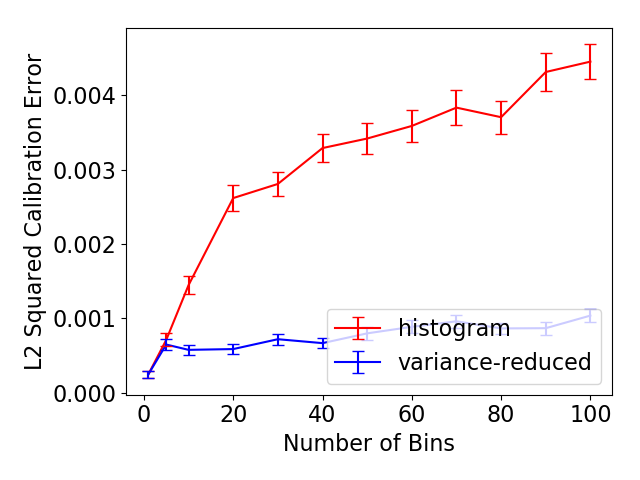
\includegraphics[width=\textwidth]{top_ces_imagenet.png}
         \caption{Effect of number of bins $B$ on top calibration error on ImageNet.
         }
         \label{fig:imagenet_top_cal_var_red}
     \end{subfigure}
     \hfill
     \begin{subfigure}[b]{0.48\textwidth}
         \centering
         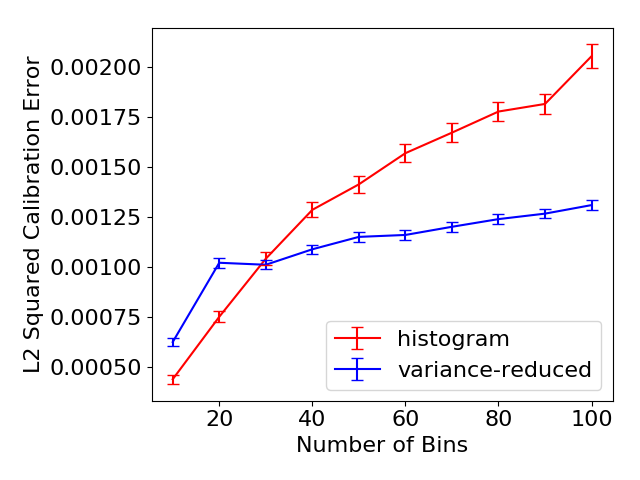
\includegraphics[width=\textwidth]{top_ces_cifar_1000.png}
         \caption{Effect of number of bins $B$ on top calibration error on CIFAR-10.
         }
         \label{fig:cifar_top_cal_var_red}
     \end{subfigure}
  \caption{
    Recalibrating using 1,000 data points on ImageNet and CIFAR-10, \ourcal{} typically achieves lower $\lsquared$ calibration error than histogram binning, especially when the number of bins $B$ is large. The difference is very significant on ImageNet, where our method does better when $B \geq 10$, and gets a nearly 5 times lower calibration error when $B = 100$. For CIFAR-10 our method does better when $B > 30$, which supports the theory, which predicts that our method does better when $B$ is large. However, when $B$ is small, practitioners should try both histogram binning and \ourcal{}.
    \pl{still need to update the legend to scaling-binning}
}
  \label{fig:mse_estimators_bins}
\end{figure}

In this experiment, we are checking a very precise hypothesis---assuming that the empirical distribution on the 10,000 validation points is the true data distribution, how do these methods perform? This is similar to the experimental protocol used in e.g.~\cite{brocker2012empirical}.
% This is not the same as an alternative hypothesis---how do these methods perform on the true CIFAR-10 distribution, which we do not have access to.
An alternative experimental protocol would have been to first split the CIFAR-10 data into two sets of size $(1000, 9000)$.
We could have then used the first set to recalibrate the model using either \ourcal{} or histogram binning, and then used the remaining 9,000 examples to estimate the calibration error on the ground truth distribution, using Bootstrap to compute confidence intervals.
However, when we ran this experiment, we noticed that the results were very sensitive to which set of 1,000 points we used to recalibrate.
Multiple runs of this experiment led to very different results.
The point is that there are two sources of randomness---the randomness in the data the recalibration method operates on, and the randomness in the data used to evaluate and compare the recalibrators.
In our protocol we account for both of these sources of randomness.

\textbf{Top-label calibration experiments}: We also ran experiments on top-label calibration, for both ImageNet and CIFAR-10. The protocol is exactly as described above, except instead of calibrating each of the $K$ classes, we calibrated the top probability prediction of the model. More concretely, for each input $x_i$, the uncalibrated model outputs a probability $p_i$ corresponding to its top prediction $k_i$, where the true label is $y_i$. We create a new dataset $\{(p_1, \mathbb{I}(k_1 = y_1)), \dots, (p_n, \mathbb{I}(k_n = y_n))\}$ and run \ourcal{} (fitting a sigmoid in the function fitting step, as in Platt scaling) or histogram binning on this dataset, using $B$ bins. This calibrates the probability corresponding to the top prediction of the model. We evaluate the recalibrated models on the top-label calibration error metric described in Section~\ref{sec:formulation}. For both CIFAR-10 and ImageNet we sampled, with replacement, a recalibration set of 1,000 points for the recalibration data, and we measured the calibration error on the entire set (10,000 points for CIFAR-10, and 50,000 points for ImageNet) as above. We show $90\%$ confidence intervals for all plots.

Figure~\ref{fig:imagenet_top_cal_var_red} shows that on ImageNet \ourcal{} gets significantly lower calibration errors than histogram binning when $B \geq 10$, and nearly a 5 times lower calibration error when $B = 100$. Both methods get similar calibration errors when $B = 1$ or $B = 5$. Figure~\ref{fig:cifar_top_cal_var_red} shows that on CIFAR-10 when $B$ is high, \ourcal{} gets lower calibration errors than histogram binning, but when $B$ is low histogram binning gets lower calibration errors. We believe that the difference might be because the CIFAR-10 model is highly accurate at top-label prediction to begin with, getting an accuracy of over $93\%$, so there is not much scope for re-calibration. In any case, this ablation tells us that practitioners should try multiple methods when recalibrating their models and evaluate their calibration error.

\textbf{(A) Synthetic experiments to validate bounds}: We first describe the scaling family we use, which is Platt scaling after applying a log-transform~\cite{platt1999probabilistic}, otherwise known as beta calibration~\cite{kull2017sigmoids}. Let $\sigma$ be the standard sigmoid function given by:
\[ \sigma(x) = \frac{1}{1 + \exp(-x)} \]
Then, our recalibration family $\mathcal{G}$ consists of $g$ parameterized by $a, c$, given by:
\[ g(z; a, c) = \sigma\Big( a\log{\frac{z}{1-z}} + c \Big) \]
In this set of synthetic experiments, we assume well-specification, that is $P(Y = 1 \mid Z=z) = g(z; a, c)$ for some $a, c$. We set $P(Z) = \mbox{Uniform}[0, 1]$. Since we know $P(Y = 1 \mid Z)$, we can approximate the true $\squaredce$ in this case, even for scaling methods. To do this, we sample $m=10000$ points $z_1, \dots, z_m$ independently from $P(Z)$. An \emph{unbiased} estimate of the $\squaredce$ then is:
\[ \squaredce(g) \approx \frac{1}{m} \sum_{i=1}^m \big[P(Y \mid Z = z_i) - g(z_i)\big]^2 \]
For each $n$ (number of recalibration samples) and $B$ (number of bins), we run either histogram binning or \ourcal{} with scaling family $\mathcal{G}$ and evaluate its calibration error as described above. We repeat this 1000 times, and compute 90\% confidence intervals. We fix $a = 2$ and $c = 1$.

\begin{figure}
  \centering
  \centering
     \begin{subfigure}[b]{0.48\textwidth}
         \centering
         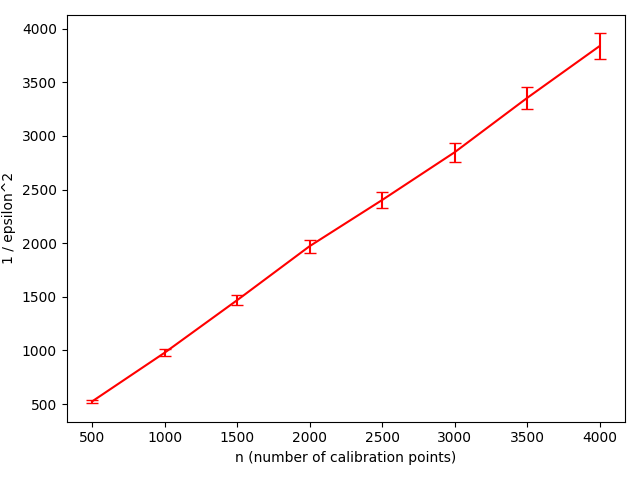
\includegraphics[width=\textwidth]{hist_vary_n_a2_b1.png}
         \caption{Histogram binning.
         }
         \label{fig:well-spec-vary-n-hist}
     \end{subfigure}
     \hfill
     \begin{subfigure}[b]{0.48\textwidth}
         \centering
         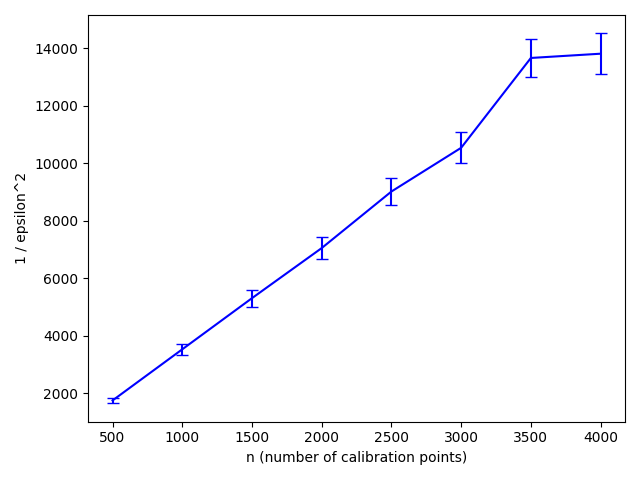
\includegraphics[width=\textwidth]{var_red_vary_n_a2_b1.png}
         \caption{\Ourcal{}.
         }
         \label{fig:well-spec-vary-n-var-red}
     \end{subfigure}
  \caption{
    Plots of $1/\epsilon^2$ against $n$ (recall that $\epsilon^2$ is the $\lsquared$ calibration error). We see that for both methods $1/\epsilon^2$ increases approximately linearly with $n$, which match the theoretical bounds.
    \tnote{does it make sense to make this two plots have the same y limit? Or we could even put the two curves one the same figure?}
}
  \label{fig:well-spec-vary-n}
\end{figure}

In the first sub-experiment we fix $B = 10$ and vary $n$, plotting $1/\epsilon^2$ in Figure~\ref{fig:well-spec-vary-n} (recall that $\epsilon^2$ is the $\lsquared$ calibration error). We plot the calibration errors for each method in a different plot because of the difference in scales, \ourcal{} achieves a much lower calibration error than histogram binning. As the theory predicts, we see that $1/\epsilon^2$ is approximately linear in $n$ for both calibrators. For example, when $B=10$ if we increase from $n=1000$ to $n=2000$ the $\lsquared$ calibration error of histogram binning decreases by $2.00 \pm 0.06$ times, and the $\lsquared$ calibration error of our method decreases by $1.98 \pm 0.09$ times.

\begin{figure}
  \centering
  \centering
     \begin{subfigure}[b]{0.48\textwidth}
         \centering
         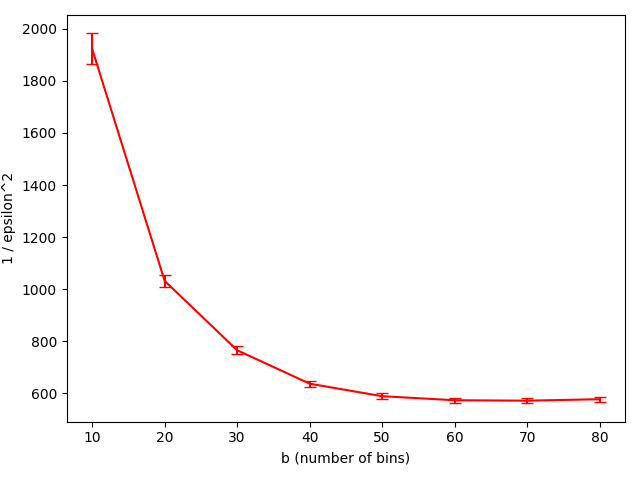
\includegraphics[width=\textwidth]{hist_vary_b_a2_b1.png}
         \caption{Histogram binning.
         }
         \label{fig:well-spec-vary-b-hist}
     \end{subfigure}
     \hfill
     \begin{subfigure}[b]{0.48\textwidth}
         \centering
         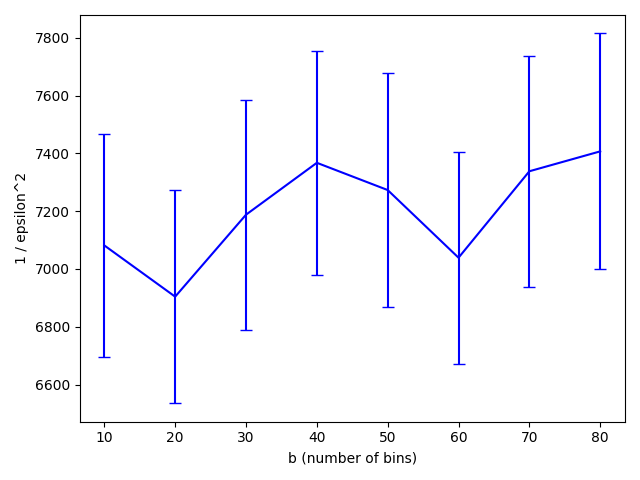
\includegraphics[width=\textwidth]{var_red_vary_b_a2_b1.png}
         \caption{\Ourcal{}.
         }
         \label{fig:well-spec-vary-b-var-red}
     \end{subfigure}
  \caption{
    Plots of $1/\epsilon^2$ against $b$ (recall that $\epsilon^2$ is the $\lsquared$ calibration error). Note that the $Y$ axis for \ourcal{} is clipped to 6600 and 7800 to show the relevant region. We see that for histogram binning $1/\epsilon^2$ scales close to $1/B$, in other words the calibration error increases with the number of bins (important note: the plot decreases because we plot the inverse $1/\epsilon^2$). For \ourcal{} $1/\epsilon^2$ is relatively constant, within the margin of estimation error, as predicted by the theory.
    \tnote{similar comments to the those for the figure above}
}
  \label{fig:well-spec-vary-b}
\end{figure}

In the second sub-experiment we fix $n = 2000$ and vary $B$, plotting $1/\epsilon^2$ in Figure~\ref{fig:well-spec-vary-b}. For \ourcal{} $1/\epsilon^2$ is nearly constant (within the margin of error), but for histogram binning $1/\epsilon^2$ scales close to $1/B$. When $n = 2000$ and we increase from $5$ to $20$ bins, our method's $\squaredce$ decreases by $2\% \pm 7\%$ but for histogram binning it increases by $3.71 \pm 0.15$ \emph{times}. For reference, we plot $P(Y \mid Z = z)$ in Figure~\ref{fig:well-spec-curve}.

\begin{figure}
  \centering
  \centering
     \begin{subfigure}[b]{0.48\textwidth}
         \centering
         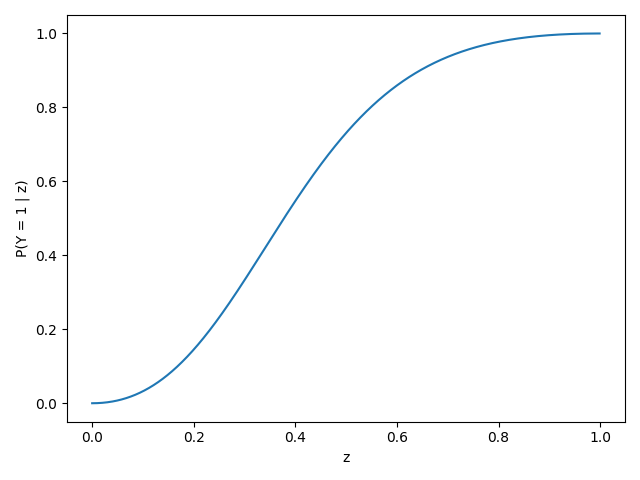
\includegraphics[width=\textwidth]{curve_a2_b1.png}
         \caption{$P(Y \mid Z=z)$ for Experiment (A)
         }
         \label{fig:well-spec-curve}
     \end{subfigure}
     \hfill
     \begin{subfigure}[b]{0.48\textwidth}
         \centering
         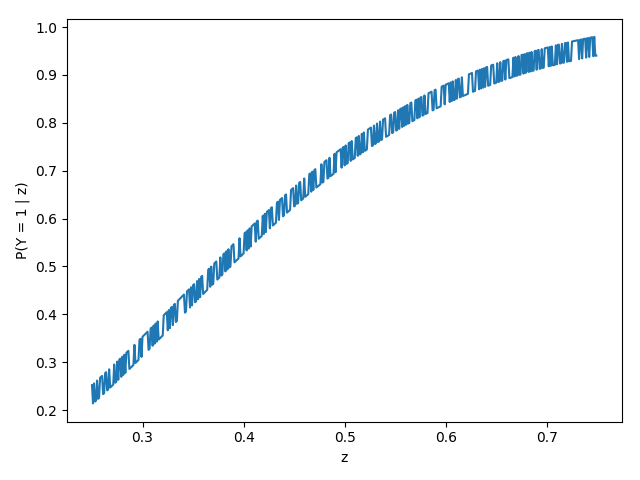
\includegraphics[width=\textwidth]{noise_curve_a2_b1.png}
         \caption{$P(Y \mid Z=z)$ for Experiment (B)
         }
         \label{fig:noisy-spec-curve}
     \end{subfigure}
  \caption{
    Plots of $P(Y \mid Z=z)$ against $z$ for both synthetic experiments.
}
  \label{fig:p_y_z_plots}
\end{figure}


\textbf{(B) Synthetic experiments to compare \ourcal{} and the scaling method}: We run an illustrative toy experiment to show that there are some cases where \ourcal{} does better than the underlying scaling method---there are other cases where the underlying scaling method does better. \ourcal{} can do better because if we have infinite data, Proposition~\ref{prop:bin_low_bound} showed that the binned version $g_{\bins{}}$ has lower calibration error than $g$. On the other hand, in step 3 of \ourcal{} algorithm we empirically bin the outputs of the scaling method which incurs an estimation error, and could mean \ourcal{} has higher calibration error than the underlying scaling method. Our key advantage is that unlike scaling methods our method has measurable calibration error so if we are not calibrated we can get more data or use a different scaling family.

Building on the previous synthetic experiments, in this experiment, we set the ground truth $P(Y = 1 \mid Z=z) = g(z; a, c) + h(z)$ where for each $z$, $h(z) \in \{-0.02, 0.02\}$ with equal probability. In this case we set $P(Z) = \mbox{Uniform}[0.25, 0.75]$ so that $P(Y = 1 \mid Z=z) \in [0, 1]$. We fix $B=10$ and vary $n$, plotting the $\lsquared$ calibration error $\epsilon^2$ in Figure~\ref{fig:well-spec-vary-b}. With $B=10$ bins, $n = 3000$ the $\lsquared$ calibration error is $5.2 \pm 1.1$ times lower for \ourcal{} than the underlying scaling method using a sigmoid recalibrator. For reference, we plot $P(Y \mid Z = z)$ in Figure~\ref{fig:noisy-spec-curve}.

\begin{figure}
  \centering
  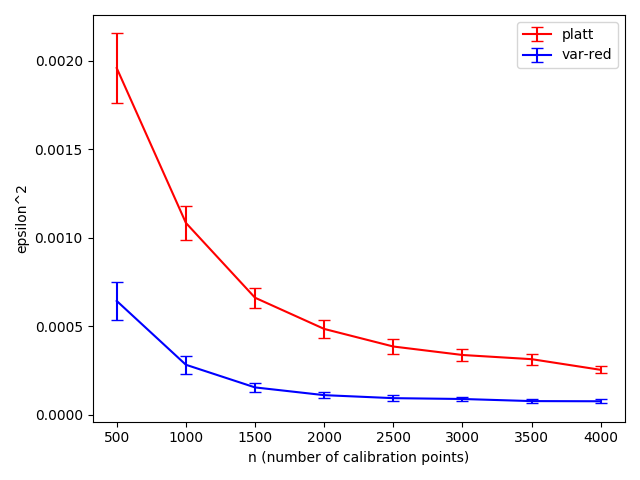
\includegraphics[width=0.6\textwidth]{noise_vary_n_a2_b1.png}
  \caption{Plot of $\epsilon^2$ ($\lsquared$ calibration error) against number of samples $n$ used to recalibrate. We can see in this case \ourcal{} consistently gets lower calibration error.
  }
  \label{fig:well-spec-vary-b}
\end{figure}
